Corresponding to each chromosome, this thesis propose an improved \gls{aco} algorithm that plays the fitness evaluation role as well as finds the shortest path from the source node to the target node. 
%In the beginning, the trail intensity on all routes was initialized equally and regularly with a small value. Subsequently, the algorithm iterates itself until it accomplishes the termination criteria. This process consists of the following sequential stages: In the first stage, the ants start from their nest and find their way. 

To travel from node $v_i$, the $k^{th}$ ant must choose an edge $e$ in the $Adj(v_i)$ through a transition probability function (Equation~\ref{equation:edge_pick}).

\begin{algorithm}
	%\setstretch{0.9}
	\caption{Ant's Pathfinding Algorithm (APA)}
	\label{alg:apa}
	\textbf{Input}:	
	\begin{itemize}
		\item A filtered multi-graph $G' = (V', E', w, s, t)$;
		\item An individual $I = (\pi_1, \pi_2,...,\pi_{|D|})$;
	\end{itemize}
	\textbf{Output}: A path $p = \{s, p_1, \dots, t\}$ and its cost. \\
	\Begin
	{	
		$D_{visited} \leftarrow\emptyset$ \Comment{List of visited domains}\;
		$visited[v] \leftarrow false~\forall v \in V$ \Comment{List of visited nodes}\;
		$cur \leftarrow s$ \Comment{The node that ant $k$ is visiting}\;
		$d \leftarrow  -1$ \Comment{The edge's domain that $p$ is visiting}\;
		\tcc{c(v) is the cost from s to v}
		$c(s) \leftarrow 0$, $c(t) \leftarrow \infty$;\\
		\While{$cur \neq t$}
		{
			$visited[cur] \leftarrow true$\;
			$Adj(cur) \leftarrow$ The set of edges that connect $v$ to other unvisited nodes in $G'$, in which each edge must satisfy the $Checksum$, $Domain~Blacklist~Check$, and its domain is not in $D_{visited}$\;
			%			$Adj(cur) \leftarrow$ Construct set of candidate edges 
			% \Comment{Refer to Algorithm~\ref{alg:edge-set}}\;
			\If{$Adj(cur) = \emptyset$}{ break\;}
			\If{$k$ is dull ant}{
				$e \leftarrow$ Choose an edge based on its attractiveness\;
			}
			\Else{
				Calculate the probability of moving to each edge as Equation (1)\;
				$e \leftarrow$ Choose an edge by $Roulette~Selection$\;
			}
			$d' \leftarrow$ the domain of $e$\;
			\If{$d \neq -1~and~d' \neq d$}{
				$D_{visited} \leftarrow D_{visited} \cup \{d\}$
			}
			$d \leftarrow d'$; $c(v) \leftarrow c(cur) + w(e)$;  $cur \leftarrow v$\; 
		}
		\Return $p$ and $c(t)$\;
	}
\end{algorithm}


\begin{equation}
	\label{equation:edge_pick}
	p_e(t) = 
	\frac{[\tau_e(t)]^{\alpha} \cdot [\eta_e(t)]^{\beta} \cdot  [P_e(t)]^{\gamma}}{\Sigma_{h \in Adj(v_i)} [\tau_h(t)]^{\alpha} \cdot [\eta_h(t)]^{\beta} \cdot [P_h(t)]^{\gamma}},
\end{equation}

\subsubsection{Ant Colony Optimization with Dull Ants}
Typically, traditional \gls{aco} approaches have a potential drawback of premature convergence to a local optimum, often caused by a large amount of pheromone deposited by previous ant generations. Together with minimizing the impact of this phenomenon, we add a new type of ant, called $dull~ant$~\cite{shimomura2010ant}, to the colony. The notable feature of dull ant is that while it can neither trail the pheromone nor perceive the domains' priority, it can still deposit the pheromone. Therefore, dull ants will not be affected by other ants, opening up opportunities to discover alternatively better paths.

\subsubsection{Checksum}
To ease the search for each ant, we employ a second component, coined $Checksum$. Before choosing an edge $e$, ant $k$ will sum its current path length and the weight of $e$. If this sum is greater than the currently found best solution, $e$ is removed from the candidate edge set. Checksum not only expedites the ant's search process but also ensures that the solution located will always be better than the previous one.

\subsubsection{Blacklist of Domains on each Node}
One problem encountered when applying \gls{aco} to incomplete graphs is that ant gets stuck at a specific node since there is no subsequent path. Moreover, this phenomenon transpires more frequently in \gls{idpcdu}, where ant not only finds a path, but the path must also fulfill the \gls{du} constraint. In other words, a domain sequence is deemed to be stuck when an ant is unable to find any edges satisfying the \gls{du} constraint leading to one of the subsequent nodes. To remedy this shortcoming, we propose an anti-stuck strategy for multi-domain problems like \gls{idpcdu}. Except for the source and destination, every time an ant arrives at a stuck node, its list of visited domains is stored in the node's blacklist. Before deciding an edge $e$, the ant checks if the edge's domain $d$ is the one that causes a stuck of any sequence of domains in the blacklist of the node to which it leads. In such a case, the ant will continue to scan whether its list of visited domains is a superset of the other after discarding $d$. Consequently, $d$ will be removed from the candidate edge set if this point is satisfied. Algorithm~\ref{alg:blacklist} presents how to check if a list of domains is in the blacklist of any node. Note that before being saved to the blacklist as well as when the ant performs the $Domain~Blacklist~Check$, the domains will be sorted in a particular predefined order. Thus, the retrieval of data is performed faster, saving both time and resources.

\begin{algorithm}
	%\setstretch{0.9}
	\caption{Domain Blacklist Check}
	\label{alg:blacklist}
	\textbf{Input}:	
	\begin{itemize}
		\item A list of domains $LD$;\\
		\item A blacklist $blacklist^v$ of node $v$;\\
	\end{itemize}
	\textbf{Output}: $LD$ is in $blacklist^v$ or not.\\
	\Begin
	{	
		$d \leftarrow $ the last element in $LD$\;
		$LD' \leftarrow LD$ without $d$\;		
		\ForEach{list of domains $LD_i$ in $blacklist^v$}
		{
			$d_i \leftarrow $ the last element in $LD_i$\;
			\If{$d = d_i$}
			{
				$LD_i' \leftarrow LD_i$ without $d_i$\;
				\If{$LD_i' \subseteq LD'$} {\Return true\;}
			}
		}
		\Return false\;
	}
\end{algorithm}

\setlength{\intextsep}{3pt}
\renewcommand{\scalefigure}{0.9}
\begin{figure}[htbp]
	\centering
	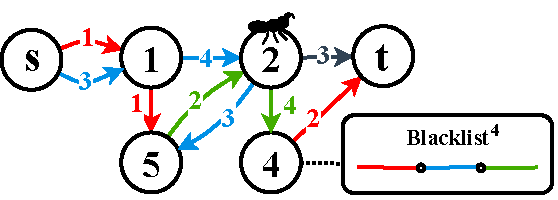
\includegraphics[scale=\scalefigure]{Figures/chap 3/BlacklistV2.pdf}
	\caption{An example of an ant checking the blacklist}
	\label{fig:blacklist}
\end{figure}

Take Figure~\ref{fig:blacklist} as a sample blacklist implementation in ant's route selection. Suppose that the blacklists of all nodes are initially empty, and an edge that goes from node $i$ to $j$ with an associated weight $w$ and belongs to domain $d$ is denoted by $(i, j, w, d)$. The first ant starts from $(s, 1, 1, red)$, $(1, 2, 4, blue)$, $(2, 4, 4, green)$ and gets stuck at node 4 because it can only revisit the $red$ domain. Therefore, the order of domains $(red, blue, green)$ is added to the blacklist of node 4. The next ant has the same beginning as the previous one. When standing at node 2, it realizes that there is only one route $(2, 4, 4, green)$, which also belongs to the domain that caused the stuck at node 4. The ant then resumes checking and finds that its visited domains list is also the stuck list without the $green$ domain. Therefore, the ant will remove this edge from the candidate set and select another. An ant has the following path $(s, 1, 3, blue)$, $(1, 5, 1, red)$, $(5, 2, 2, green)$. When it reaches node 2, it does the same thing as the second ant. In this case, its traversed domains list is a superset of the one after discarding the $green$ domain, and in the end, the edge $(2, 4, 4, green)$ is still eliminated. This strategy allows the searching candidate edge of ant more thoroughly without saving a plethora of stuck cases. The shorter the order of domains in blacklists, the more effective this method will be.